\documentclass[a4paper,11pt]{style/uneceart}

\usepackage{style/UNECE2025}
\usepackage{enumerate}
\usepackage[T1]{fontenc}      % proper font encoding
\usepackage[table]{xcolor}
\definecolor{unece_color}{RGB}{84, 141, 212}
\usepackage{booktabs}
\usepackage{rotating} % Rotating table
\usepackage{subcaption}
\usepackage{graphicx}
\usepackage{multirow}
\usepackage{amsmath}
\usepackage{array} % necessary for word wrap within a table

%%% ----------------------------------------------------------------------
%%% ---   please fill-in your personal data:   ---------------------------

%% the title of your contribution in capital letters:
\newcommand{\TITLE}{\textbf{Buyer Beware: Understanding the trade-off between utility and risk in CART based models using simulation data} \\}

%% author:
\newcommand{\AUTHOR}{Jonathan Latner$^{1}$, Marcel Neunhoeffer$^{1,2}$, J\"{o}rg Drechsler$^{1,2,3}$}

%% your organisation
\newcommand{\ORGANISATION}{\vspace{2mm} \\  $^{1}$Institute for Employment Research, Nuremberg, Germany \\ 
$^{2}$Ludwig-Maximilians-Universit\"at, Munich, Germany \\ 
$^{3}$University of Maryland, College Park, USA
}
\newcommand{\EMAIL}{jonathan.latner@iab.de}

%% abstract
\newcommand{\ABSTRACT}{This paper evaluates disclosure risk measures for synthetic data generated by CART-based models, using both a controlled simulated dataset and publicly available data. We find that common disclosure risk measures may fail to detect disclosure risks and, in some cases, misrepresent actual disclosure risks. Additionally, CART-based models, while maintaining high statistical utility, may compromise privacy protection. Our findings highlight challenges in measuring disclosure risk of synthetic data and suggest improvements for more accurate risk assessments.}


\begin{document}
%% Cover page with title and abstract
%%% Updated

\setcounter{page}{1}
\thispagestyle{empty} \vspace*{-2.0cm} %[width=0.65\textwidth]

\includegraphics[height=1.5cm]{UNECE_logo}\hspace*{8cm}
\includegraphics[height=1.5cm]{ModernStatsLogo}\\[\baselineskip]
%\hspace*{13cm} Working Paper \\
%\hspace*{13cm}ENGLISH ONLY\\\\
\textsc{UNITED NATIONS ECONOMIC COMMISSION FOR EUROPE} \vspace*{2mm}\\
\textsc{CONFERENCE OF EUROPEAN STATISTICIANS}\vspace*{2mm}\\
\textbf{Expert meeting on Statistical Data Confidentiality}\vspace*{2mm}\\
15--17 October 2025, Barcelona              %% check whether it is the right place and date
\vspace*{-1mm}
{\color{unece_color} \par\noindent\rule{\textwidth}{1.25pt}}\\[1cm]
%\TOPIC
%\begin{center}
{\LARGE \TITLE}\vspace*{-2mm}\\ %17pt
%\TYPE
\AUTHOR\ %11pt
\ORGANISATION\vspace{2mm}\\ %11pt
\EMAIL\vspace*{1cm}\\ %11pt
%\end{center} 
\noindent
{\large\textbf{\textit{Abstract}}}\\ %12pt
\ABSTRACT
\newpage



\title{Buyer Beware: Understanding the trade-off between utility and risk in CART based models using simulation data}

\section{Introduction}

In this paper, we ask whether commonly used privacy measures accurately capture disclosure risk in synthetic data generated by CART\footnote{CART stands for classification and regression trees \citep{breiman2017classification}.}-based models. The generation of synthetic data has gained prominence as a means to share data while preserving privacy. There are numerous methods and tools, both for generating synthetic data and measuring privacy.  On the one hand, there is a general perception that generating synthetic data are easy \citep{latner2024generating}, and to a certain degree this is true.  On the other hand, it is not always clear if the resulting synthetic data are in fact providing privacy protection, especially if no formal privacy methods are used.

We evaluate standard and easily available privacy measures to estimate risk from synthetic data generated by CART-based models.  We use CART because previous research indicates that CART-based synthetic data generators (SDGs) generate synthetic data with both high statistical utility and relatively low privacy risks compared to other methods \citep{little2025synthetic,fossing2024evaluation,dankar2021fake}.  In addition, we use two measures of disclosure risk: identity disclosure risk and attribute disclosure risk \citep{raab2025practicalprivacymetricssynthetic}.  While some argue that privacy is a property of the algorithm that created the synthetic data, not the synthetic data itself \citep{jordon2022synthetic}, these measures reflect the current state of the art in the evaluation of statistical disclosure control in synthetic data \citep{raab2025practicalprivacymetricssynthetic}.  Empirical disclosure risk measures are also recommended for synthetic data generated using formal privacy guarantees, as it may be hard to translate the formal guarantees into practical language \citep[see, e.g.,][]{desfontainesblog20250407}.  Therefore, our results have broader relevance, contributing to our understanding of both the evaluation of privacy risk measures and the assessment of synthetic data generators.

We use both simulated and real survey data for our analysis. The simulated data repliacte a design by \citet{reiter2014bayesian}, consisting of 1.000 observations and four binary variables. Crucially, the last or 1.000$^{th}$ observation is a unique combination of the four binary variables.  In so doing, we create data with an observation we want to protect using synthetic data generated from a CART model.  We also use publicly available data from Social Diagnosis 2011 (SD2011) to extend our analysis beyond a simulated setting and into a real-world setting.

Our approach follows a structured framework. Using the simulated data and drawing on concepts from the attack model in differential privacy, we estimate risk measures for an attacker with full knowledge of the synthetic data generator, all synthetic observations, and all original observations except the disclosive record.  First, we test whether an attacker can identify the disclosive record.  They can.  Next, we test whether the privacy measures detect a known disclosure risk in the simulated data. They do not.  Finally, we extend the analysis using the SD2011 data to assess whether the measurement problem is specific to the simulated case or part of a broader challenge in detecting privacy risk. The results suggest the latter.

Conditional on the assumption of a strong attacker model, we make three contributions.  Commonly used disclosure risk measures both may not capture disclosure risk in a way that a user would expect. We show this result using synthetic data generated from simulated data, and also show how these measures may misstate privacy risks in real data.  Further, relatedly, and in contrast to previous research, CART-based models may produce synthetic data that sacrifices privacy protection for statistical utility.  Finally, we propose some solutions for measuring disclosure risk.  More generally, users interested in measuring privacy risk should be aware of the challenges we describe here.

\section{Disclosure risk measures}

While the literature on privacy measures for statistical computations is well-developed \citep{wagner2018technical}, the literature on disclosure risk measures for synthetic data is relatively sparse.  With regards to synthetic data, there is currently no one agreed upon understanding of either what defines a disclosure risk nor how one should measure it. In this paper, we evaluate two commonly used measures of disclosure risk implemented in the popular Synthpop package \citep{nowok2016synthpop} in R  \citep{raab2025practicalprivacymetricssynthetic}: identity disclosure risk and attribute disclosure risk.  
We also evaluate a third measure of disclosure risk based on Bayesian estimation, first proposed by \citet{reiter2014bayesian}.

\subsection{Identity disclosure risk} 
Identity disclosure risk measures the ability to identify individuals in the data from a set of known characteristics, i.e. `keys'. The maximum number of keys are one less than the total number of variables in the data.  

The following steps are used to calculate identity disclosure risk.  For a given set of keys ($q$), the intruder will look for the unique records in the original data ($UiO$) that are also unique in the synthetic data ($UiS$).  $repU$ (replicated uniques) is the measure of identity disclosure risk and defined by equation \ref{eq:repU}:

\begin{equation}
repU = 100 \sum (s_{.q}|d_{.q} = 1 \land s_{.q} = 1 )/N_{d}
\label{eq:repU}
\end{equation}

where $d_{.q}$ is the count of records in the original data with the keys corresponding to a given value of $q$ and $s_{.q}$ is the equivalent count for the synthetic data.  In a given value of $q$, $s_{.q}|d_{.q} = 1$ is a unique record in the original data conditional on also existing in the synthetic data.  $s_{.q} = 1$ is the unique record in the synthetic data.  This is summed over all unique values of $q$ and divided by the total number of records in the data ($N_{d}$) and multiplied by 100 to transform the ratio into a percentage.

We do not believe that this is a good measure of identity disclosure risk and empirically show in Section \ref{sec:results} that it fails to ring an alarm in a case where an identity is disclosed by synthetic data.

\subsection{Attribute disclosure risk} 
Attribute disclosure risk measures the ability to identify a previously unknown characteristic of an individual.  In this approach, an attacker has access to synthetic data, knows one or more identifiers in the original data (i.e. $q$ or keys, as above), and wants to infer a sensitive attribute ($t$).  Attribute disclosure risk or $DiSCO$ (Disclosive in Synthetic Correct in Original) is the subset of records in the original data for which the keys ($q$) in the synthetic data are disclosive. $q$ is disclosive if all records in the synthetic data with the same $q$ have a constant target ($t$), i.e. no variation in $t$, as defined by the following equation \ref{eq:DiSCO}:

\begin{equation}
DiSCO = 100 \sum^{q} \sum^{t} (d_{tq} | ps_{tq} = 1) / N_{d}
\label{eq:DiSCO}
\end{equation}

where $ps_{tq} = s_{tq}/s_{.q}$ are the column proportions, and $d_{tq} | ps_{tq} = 1$ indicates whether the synthetic data matches the original data for the combination of $t$ and $q$ given the condition that the synthetic data for the combination of $t$ and $q$ is disclosive (i.e., target $t$ is uniquely determined by the keys $q$).  This is summed over unique values of $t$ and unique values of $q$ and divided by the total number of records in the data ($N_{d}$) and multiplied by 100 to transform the ratio into a percentage.

Again, we do not believe that this is a good measure of attribute disclosure risk and empirically show in Section \ref{sec:results} that it fails to ring an alarm in a case where the value of an attribute is disclosed by synthetic data.

\subsection{Bayesian estimation of disclosure risk}

A more informative way to evaluate disclosure risk is to adopt a Bayesian perspective, as suggested by \citet{reiter2014bayesian}. Essentially, the goal is to measure what an intruder with some prior distribution over potential original data sets can learn about the original data from the release of a synthetic data set. In a fully synthetic scenario, \citet{reiter2014bayesian} assume that an intruder wants to find out the values $y_i$ for one observation (i.e., the entire row) in the original database $D$. \citet{reiter2014bayesian} further assume that the intruder knows all other records in the database $D_{-i}$ and the data synthesis algorithm $S$. Given the released synthetic data set ($Z$), knowledge about the synthetic data generation process ($S$), and the prior distribution over the sample space of all possible values of $y_i$ ($p(Y_i|D_{-i}, S)$), the intruder wants to estimate the Bayesian posterior distribution for $Y_i$:

\begin{equation*}
    p(Y_i|Z,D_{-i},S) \propto p(Z|Y_i, D_{-i}, S)p(Y_i|D_{-i}, S)
\end{equation*}

From the posterior distribution, a variety of disclosure risk measures can be computed. For example, for a data set where all columns contain discrete values \citet{reiter2014bayesian}, calculate the probability that the unknown record is one specific combination of values $c_s$ out of all $K$ possible combinations $c_K$ as their measure of disclosure risk for a vulnerable record:

\begin{equation}\label{eq:bayesian}
p(Y_i = c_s|Z, D_{-i}, S) = \frac{p(Z|Y_i = c_s, D_{-i}, S)p(Y_i=c_s|D_{-i}, S)}{\sum_{k=1}^Kp(Z|Y_i = c_k, D_{-i}, S)p(Y_i=c_k|D_{-i}, S)}
\end{equation}

If this probability is close to the prior (e.g., a uniform prior would be $1/K$), then an attacker cannot learn much about the last record from the released synthetic data. However, if the attacker learns something about the original data from the released synthetic data, this probability will be larger than the prior. In the worst case, the attacker can identify the last record with certainty when $p(Y_i = c_s|Z, D_{-i}, S) = 1$.

In this paper, we show how this measure can be applied to CART-based synthesis models. At least, for simple data sets\footnote{Where $K$ is the number of possible records for each observation, which is relatively small. In our example in \ref{sec:data} $K = 16$.} like the one we look at in section \ref{sec:data}. 

However, this measure of disclosure risk is rarely used in practice as it is complicated to calculate, especially for more complex real-world data sets\footnote{As $K$ grows exponentially with the number of columns and possible values per column.}.

\section{Data}\label{sec:data}

To examine our question of interest, we use two types of data: simulated and real data.  Following \citet{reiter2014bayesian}, we simulate one data set with $1000$ observations and four binary variables.  This is our `original' data set.  The first 999 records are sampled from a multinomial distribution for all $15$ combinations of var1(0,1), var2(0,1), var3(0,1), var4(0), except the last 1000$^{th}$ record is a unique combination (var1 = 1, var2 = 1, var3 = 1, var4 = 1).  Next, we generate one synthetic data set from a CART-based SDG using the Synthpop package in R\footnote{We use the default settings and hyperparameter values as suggested by the package and set a seed=$1237$.}.  As a sensitivity test, we create 10 synthetic data sets from the original data.  The value of the simulated data is that we know there is a unique record because we created it.

At the same time, an obvious critique is that the simulated data set is not representative of real world data.  We agree with this critique, even though the value of the simulated data is to illustrate the limits of empirical disclosure risk measures in an, admittedly, edge case.  Therefore, we also use a second data set from Social Diagnosis 2011 (SD2011), publicly available from the Synthpop package in R to further examine our question of interest using real world data.

\section{Results from simulated data}\label{sec:results}

We begin with the simulated data that contains four categorical variables and $1000$ observations, one of which is unique or disclosive. For both the original and synthetic data, figure \ref{fig:frequency_compare} shows the frequency distribution within each of the four variables and figure \ref{fig:histogram_compare} the frequency histogram across all four variables.  In the original data, there is one observation with a combination (1,1,1,1) that is not visible if we look at the distribution within each of the variables.  

\begin{figure}[!h]
    \centering
    \caption{Compare original and synthetic data}
    \begin{subfigure}{0.48\textwidth}
        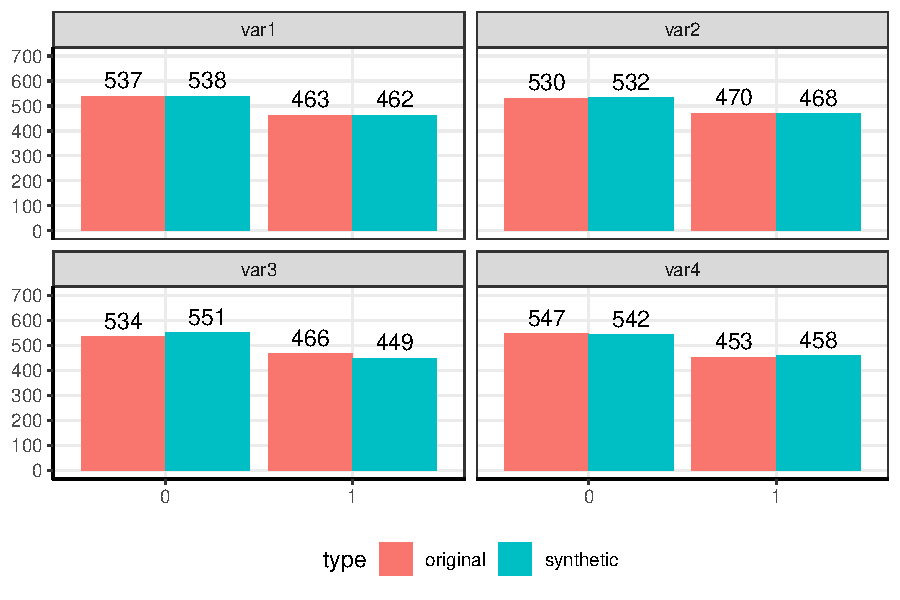
\includegraphics[width=\textwidth]{../../graphs/graph_cart_frequency_compare.pdf}
        \caption{Frequency}
        \label{fig:frequency_compare}
    \end{subfigure}
    \hfill
    \begin{subfigure}{0.48\textwidth}
        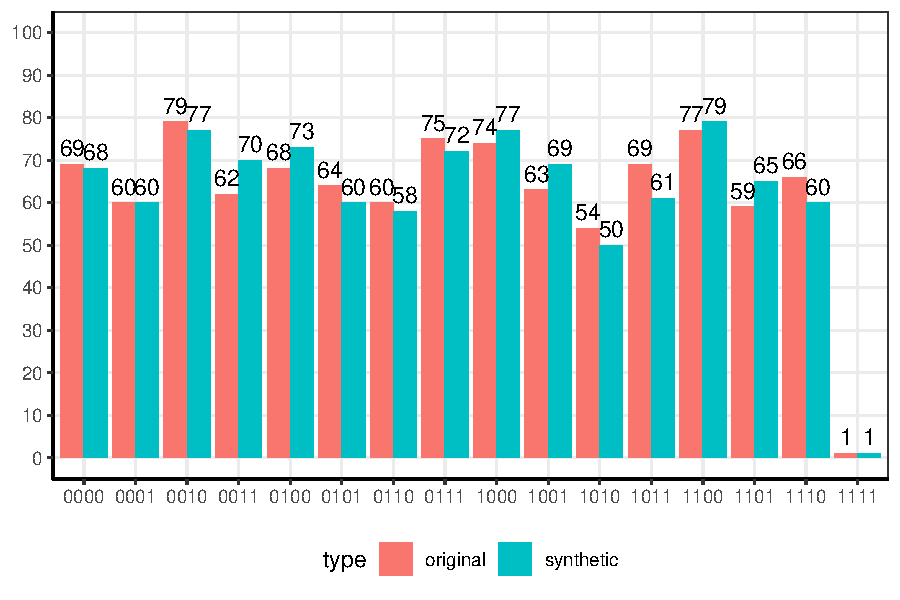
\includegraphics[width=\textwidth]{../../graphs/graph_cart_histogram_compare.pdf}
        \caption{Histogram}
        \label{fig:histogram_compare}
    \end{subfigure}
    \label{fig:compare}
\end{figure}

The synthetic data generated by the CART model have high levels of utility because they almost perfectly match the frequency of values in the original data not only within the four variables but also across all four variables. 

Looking at our known unique record in the synthetic data, the unique records reappears at least once in most of the synthetic data sets as shown in figure \ref{fig:cart_histogram_compare_10}.  The frequency of the unique record reappearing in the synthetic data ranges from 0 (in 2 out of the 10 synthetic data sets), 1 (in 5 out of the 10 synthetic data sets), 2 (in 1 out of the 10 synthetic data sets), to 3 (in 2 out of the 10 synthetic data sets).\footnote{For reference, the frequency of the unique record reappearing in the synthetic data would be similar if we created 100 synthetic data sets, ranging from 0 (41 data sets), 1 (38 data sets), 2 (14 data sets), to 3 (7 data sets).}  

\begin{figure}[!h]
    \centering
    \caption{Frequency}
    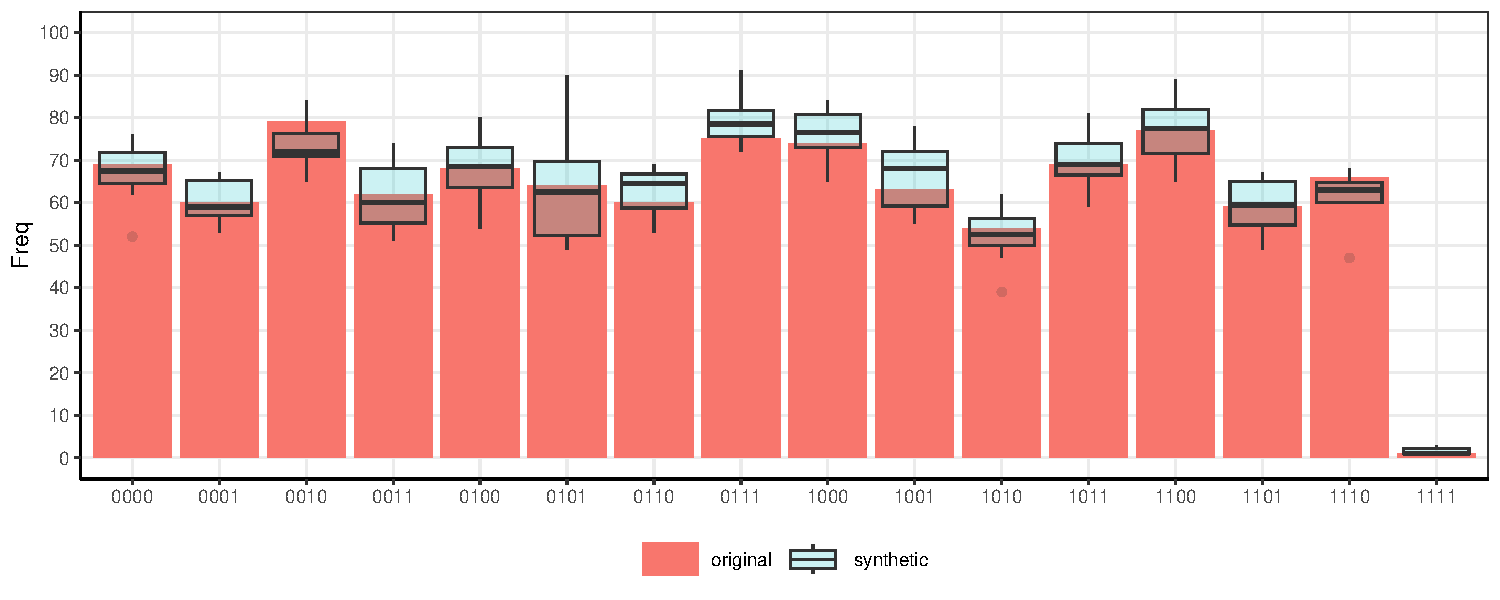
\includegraphics[width=\textwidth]{../../graphs/graph_cart_histogram_compare_10_v1.pdf}
    \label{fig:cart_histogram_compare_10}
\end{figure}


\subsection{The attack}

One way to think about disclosure risk is to imagine a game between two entities.  On one side, there is a statistical agency who has the data and wants to release it, preferably in a privacy preserving way.  On the other side, there is an attacker who wants to learn something from the release that they did not know previously (e.g., either membership or attribute inference). The question is what can the attacker learn from a released synthetic data set about an individual they do not have knowledge of?

In this scenario, we assume a strong attacker, similar to the attack model used in differential privacy (DP) \citep{dwork2006calibrating}. The attacker is assumed to know the exact SDG used to generate the synthetic data, which in our case is sequential CART\footnote{Where the attacker also knows the sequence of the sequential modeling.}, and to have access to all records in the original data except the final one. Moreover, given the small domain of the variables, the attacker knows that the last record must be one of the 16 possible combinations of the four binary variables. In this attack, the attacker sees the released synthetic dataset and generates synthetic data using the same sequential CART procedure for each of the 16 possible completed data sets. By comparing the resulting synthetic datasets with the released one, the attacker updates their posterior beliefs about which of the 16 candidate records is most likely the true one. In fact, this illustration of the attack is what \citet{reiter2014bayesian} describe as their Bayesian estimation of disclosure risk.

Figure \ref{fig:attacker_default} illustrates the results of the attack.  In the top left cell, the attacker guesses that the last record in the original data is 0,0,0,0.  They then generate 10 synthetic data sets using a CART-based SDG and compare the histogram to the released synthetic data, as shown in figure \ref{fig:cart_histogram_compare_10}.  

\begin{figure}[!h]
    \centering
    \caption{Histogram of 16 worlds x 10 synthetic datasets}
    \resizebox{\textwidth}{!}{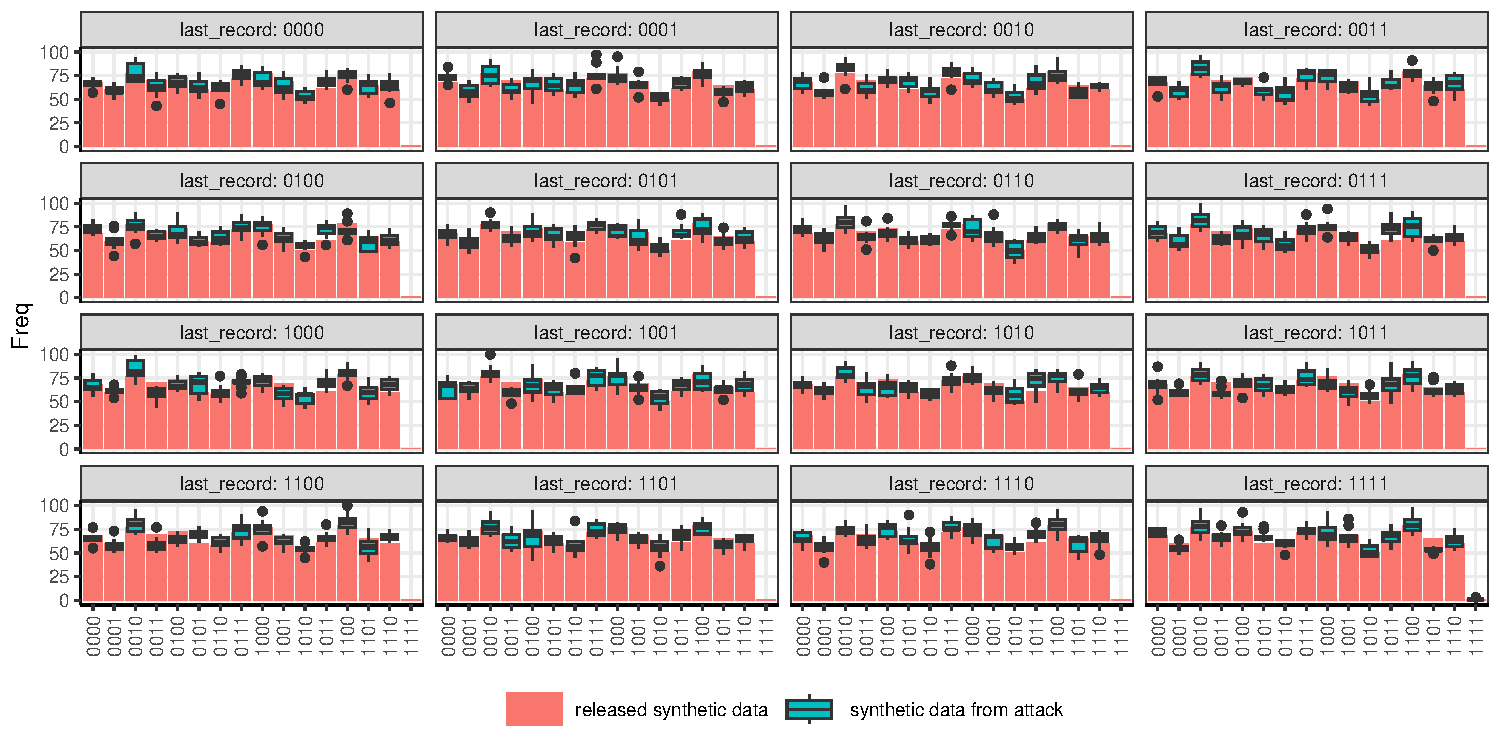
\includegraphics{../../graphs/graph_attacker_default_v1.pdf}}
    \label{fig:attacker_default}
\end{figure}

If the attacker guesses that the last record is 0, 0, 0, 0, then they are not able to replicate the record 1, 1, 1, 1 to reappear in any of the synthetic data sets.  Next, they iterate through all 16 potential original data sets. 

What we see in Figure \ref{fig:attacker_default} is that only if they guess that the last record is 1, 1, 1, 1, then they are able to generate synthetic data with the combination 1, 1, 1, 1 reappearing, as shown in the bottom, right cell.  The result is a successful attack where the attacker can clearly distinguish what the original data set must have looked like. Conditional on observing the record 1, 1, 1, 1, in the released synthetic data, they know with certainty what the last record must have been, as they can replicate synthetic data with that record in only one out of 16 worlds.

\subsection{Measuring disclosure risk}

The larger concern is whether we are able to measure this disclosure.  Results from our simulated data show that CART produces synthetic data that is disclosive because in our setup it never generates records that are not in the  original data set even if they could theoretically exist.  Other research also indicates that CART-based SDGs can produce synthetic data with high levels of utility because they reproduce a high proportion of the original data \citep{manrique2018bayesian}.  The question is can we measure this observable risk?

In table \ref{table:disclosure_risk_1}, the columns display the measures for identity disclosure risk($repU$ - equation \ref{eq:repU}), attribute disclosure risk ($DiSCO$ - equation \ref{eq:DiSCO}), and the Bayesian estimation of disclosure risk (equation \ref{eq:bayesian} (the columns) in the original\footnote{This is assuming that the original data would be released directly. The original data is then treated as if it were synthetic in equations \ref{eq:repU}, \ref{eq:DiSCO}, and \ref{eq:bayesian}. On a theoretical level it is questionable if the measures calculated on original data are meaningful at all. After all, if you release the original data, you disclose all of the information contained in it.} and synthetic data (the rows).  For reference, we replicated table \ref{table:disclosure_risk_1} with 10 synthetic copies from figure \ref{fig:cart_histogram_compare_10}, as shown in table \ref{table:disclosure_risk_10} in the Appendix.  Results are qualitatively similar.  

\begin{table}[]
    \centering
    \caption{Disclosure risk measures}
    % latex table generated in R 4.5.0 by xtable 1.8-4 package
% Wed Aug 13 15:48:17 2025
\begin{tabular}{lrrrr}
  \toprule
Data & Unique &  Identity Risk  & Attribute Risk  & Bayesian Estimate of Risk \\ 
 & & ($repU$) & ($DiSCO$) & \\
  \midrule
Original & 1&  0.00 & 0.00 &  1.00 \\ 
  Synthetic & 1& 0.00 & 0.00 & 1.00 \\ 
   \bottomrule
\end{tabular}

    \label{table:disclosure_risk_1}
\end{table}

The identity disclosure risk measures are zero for both the original and synthetic data. In this example, the first three binary variables ($q$) are treated as keys, although this choice is arbitrary. These three attributes yield $2^3 = 8$ possible combinations, none of which are unique in the dataset. Consequently, under the $repU$ measure, the risk of identity disclosure is zero because no record can be uniquely identified based on the chosen keys. This is not ideal, as one could conclude that it safe to release the synthetic data. However, as we show in Figure \ref{fig:attacker_default} the CART-based synthetic data is disclosive.

The attribute risk measures are also 0 for both the original and synthetic data.  Here, the target is the 4th binary variable.  This is a problem because we know that when $q=111$, there is a unique record if $t=1$.  

How can the metric report no attribute disclosure risk when we know that such a risk exists in reality? The explanation lies in how the metric is defined: it registers an attribute disclosure risk only when $t$ is constant, meaning there is no variation in $t$ within the set of records sharing the same $q$. Under this definition, the metric reports a risk only when there are zero copies of the unique record in the synthetic data. In other cases, the real possibility of attribute disclosure may still be present, but it is not captured by the metric.


We can see this issue more clearly if we examine the frequency table from 10 synthetic data copies, as shown in figure \ref{fig:cart_histogram_compare_10}.  The underlying data and resulting empirical disclosure risk measures are shown in the appendix (table \ref{table:frequency_10_data_sets} and \ref{table:disclosure_risk_10}).  If there is at least one unique record in the synthetic data, then there is no attribute disclosure risk because there are 2 values of $t$ within $q$.  At the same time, if a synthetic data set is released without the unique record, then there is an attribute disclosure risk because there is only 1 value of $t$ within $q$.  

Therefore, the attribute disclosure risk measure indicates a disclosure risk when we know there is no disclosure risk, and indicates there is no disclosure risk when we know there is a disclosure risk.  The exercise illustrates a fundamental flaw in the measure of attribute disclosure risk as defined in equation \ref{eq:DiSCO}. We know there is a disclosure problem (because we created it), but the problem is not identified by the measure.  

Finally, the measure based on the Bayesian estimation of disclosure risk as defined in equation \ref{eq:bayesian} correctly identifies the disclosive nature of the CART-based synthetic data. The probability that the final record is $c_{16} = 1, 1, 1, 1$ is $1$ for both the original and the synthetic data. As we show in table \ref{table:disclosure_risk_10} in the appendix, this is true whenever at least one record equal to $c_{16}$ reappears in the synthetic data. In this example, this is even independent of the chosen prior\footnote{As long as each of the 16 worlds has a positive prior probability.}. The probability of $1$ means that the attacker is $100\%$ certain about the last record. Only in cases where the record with $c_{16}$ does not reappear in the synthetic data, the attacker is uncertain about what the final record is. For these synthetic data sets, they even assign a low value between $2\%$ and $3\%$ (see table \ref{table:disclosure_risk_10} in the appendix). 

This measure of disclosure risk makes sense. It sounds an alarm when there is a disclosure. Whereas, when the attacker cannot learn anything about the last record, it remains silent.

\section{A real world example}

In the papers describing the disclosure risk measures implemented in Synthpop \citep{raab2024privacy,raab2025practicalprivacymetricssynthetic}, the authors generate 5 synthetic data sets to illustrate their method for measuring attribute disclosure risk by identifying values in the target variable \texttt{depress} from keys: \texttt{sex} \texttt{age} \texttt{region} \texttt{placesize}.  As described above, their preferred measure of attribute disclosure risk (DiSCO) is the set of records in the synthetic data with a constant target ($t$) for a set of keys ($q$).  In other words, there is no variation of $t$ within $q$.  In their example, attribute disclosure risk in the original data is 53\%, which is reduced to about about 9\% in the synthetic data (as shown in the table \ref{tab:attribute_risk_sd2011} appendix).  

To illustrate why it is a problem to measure attribute disclosure risk as the set of records with constant $t$ within $q$, we set $t$ as constant for all observations in all 5 synthetic data sets. The value 0 was chosen because it is the most frequent value in the variable \texttt{depress} (22\% of all records).  By definition, this reduces attribute disclosure risk, as trivially no attacker could learn anything about anyones true values of \texttt{depress}.  However, according to the measure of attribute disclosure risk used by the package, the risk increases to around 15\%.

We note that this problem is already understood and described by the package authors \citep{raab2025practicalprivacymetricssynthetic}.  They provide a parameter where a user may check for a target where a high proportion of records have one level (\texttt{check\_1way}).  However, the problem is not the package, the problem is the definition.

This exercise illustrates a flaw in the measure of attribute disclosure risk using real world data.  We modified the synthetic data by setting a constant value for the target variable: \texttt{depress} = 0.  If the measure reasonably measured attribute disclosure risk, then the risk measure should decline, but it rises.  Therefore, the attribute disclosure risk measure indicates that attribute disclosure risk increased when we know attribute disclosure risk decreased (because we decreased it).  

\section{Conclusion}

In this study, we use two data sets, one simulated data with a single disclosive record and one real-world data, to demonstrate three ideas.  First, not only do common privacy metrics not detect the disclosure risks we know exist in the simulated data, but they can also misstate the disclosure risk in real-world data.  Second, relatedly, CART-based synthetic data generators with default parameters create synthetic data with high levels of utility that reproduce the original data without protection for the dislosive record.  Therefore, CART-based models are not inherently immune to the utility-privacy trade-off.  Finally, it is possible to increase protection by adding noise to the synthetic data with simple adjustments to the default parameters, but the cost is to reduce utility.  The question is why one would reduce utility if there is no indication there was a disclosure problem?  Given these results, it is important for users interested in reducing disclosure risk to better understand not only how SDGs generate synthetic data, but also how common privacy measures work.  There is no one size fits all solution. 

\subsubsection{Acknowledgements} This work was supported by a grant from the German Federal Ministry of Research, Technology, and Space (BMFTR grant number 16KISA096) with funding from the European Union-NextGenerationEU.  Reproducible files are located here: \url{https://github.com/jonlatner/KEM\_GAN/tree/main/latner/projects/simulation}

\subsubsection{Disclosure of Interest} The authors have no competing interests to declare that are relevant to the content of this article.


%%%%%%%%%%%%%%%%%%%%%%%%%%%%%%%%
% Bibliography
%%%%%%%%%%%%%%%%%%%%%%%%%%%%%%%%

\bibliographystyle{chicago}
\bibliography{references}

%%%%%%%%%%%%%%%%%%%%%%%%%%%%%%%%
% Appendix
%%%%%%%%%%%%%%%%%%%%%%%%%%%%%%%%
\clearpage
\appendix

\section{}\label{appendix}
\setcounter{figure}{0}    
\setcounter{table}{0}    
\renewcommand*\thetable{\Alph{section}.\arabic{table}}
\renewcommand*\thefigure{\Alph{section}.\arabic{figure}}
\renewcommand{\theHfigure}{\Alph{section}.\arabic{table}}
\renewcommand{\theHtable}{\Alph{section}.\arabic{figure}}

\begin{table}[!ht]
    \centering
    \caption{Frequency statistics for original and 10 synthetic data sets}
    \rowcolors{1}{white}{lightgray}
    % latex table generated in R 4.4.0 by xtable 1.8-4 package
% Mon Dec 16 16:27:40 2024
\begin{tabular}{lrrrrrrrrrrr}
  \toprule
   & \multicolumn{1}{l}{Original} & \multicolumn{10}{c}{Synthetic Data} \\ \cmidrule(lr){3-12}
 Combine & 0 & 1 & 2 & 3 & 4 & 5 & 6 & 7 & 8 & 9 & 10 \\ 
 \midrule
0000 & 69 & 68 & 66 & 71 & 73 & 76 & 62 & 72 & 52 & 64 & 67 \\ 
  0001 & 60 & 60 & 53 & 57 & 56 & 58 & 60 & 67 & 67 & 57 & 67 \\ 
  0010 & 79 & 77 & 71 & 73 & 71 & 71 & 84 & 65 & 70 & 77 & 74 \\ 
  0011 & 62 & 70 & 51 & 56 & 68 & 63 & 55 & 74 & 57 & 68 & 52 \\ 
  0100 & 68 & 73 & 63 & 80 & 54 & 61 & 79 & 65 & 73 & 66 & 71 \\ 
  0101 & 64 & 60 & 77 & 49 & 66 & 52 & 90 & 52 & 53 & 65 & 71 \\ 
  0110 & 60 & 58 & 68 & 66 & 61 & 69 & 56 & 67 & 65 & 64 & 53 \\ 
  0111 & 75 & 72 & 91 & 86 & 81 & 80 & 77 & 82 & 77 & 75 & 72 \\ 
  1000 & 74 & 77 & 84 & 80 & 73 & 70 & 81 & 82 & 65 & 76 & 73 \\ 
  1001 & 63 & 69 & 66 & 57 & 68 & 73 & 56 & 68 & 75 & 78 & 55 \\ 
  1010 & 54 & 50 & 54 & 57 & 51 & 47 & 50 & 39 & 62 & 58 & 54 \\ 
  1011 & 69 & 61 & 59 & 77 & 71 & 66 & 69 & 75 & 69 & 68 & 81 \\ 
  1100 & 77 & 79 & 77 & 76 & 83 & 78 & 66 & 65 & 88 & 70 & 89 \\ 
  1101 & 59 & 65 & 52 & 54 & 57 & 66 & 67 & 59 & 65 & 49 & 60 \\ 
  1110 & 66 & 60 & 68 & 60 & 64 & 68 & 47 & 65 & 62 & 64 & 60 \\ 
  1111 & 1 & 1 & 0 & 1 & 3 & 2 & 1 & 3 & 0 & 1 & 1 \\ 
   \bottomrule
\end{tabular}

    \label{table:frequency_10_data_sets}
\end{table}

\begin{table}[!ht]
    \centering
    \caption{Risk measures from 10 synthetic data sets}
    \rowcolors{1}{white}{lightgray}
    % latex table generated in R 4.5.0 by xtable 1.8-4 package
% Wed Aug 13 15:48:18 2025
\begin{tabular}{lrrr}
  \toprule
Data & Identity Risk ($repU$) & Attribute Risk ($DiSCO$) & Bayesian Estimate of Risk \\ 
  \midrule
Original & 0.00 & 0.00 & 1.00 \\ 
  Synthetic 1 & 0.00 & 0.00 & 1.00 \\ 
  Synthetic 2 & 0.00 & 6.60 & 0.02 \\ 
  Synthetic 3 & 0.00 & 0.00 & 1.00 \\ 
  Synthetic 4 & 0.00 & 0.00 & 1.00 \\ 
  Synthetic 5 & 0.00 & 0.00 & 1.00 \\ 
  Synthetic 6 & 0.00 & 0.00 & 1.00 \\ 
  Synthetic 7 & 0.00 & 0.00 & 1.00 \\ 
  Synthetic 8 & 0.00 & 6.60 & 0.03\\ 
  Synthetic 9 & 0.00 & 0.00 & 1.00 \\ 
  Synthetic 10 & 0.00 & 0.00 & 1.00 \\ 
  Average & 0.00 & 1.32 & - \\ 
   \bottomrule
\end{tabular}

    \label{table:disclosure_risk_10}
\end{table}


\begin{figure}[!h]
    \centering
    \caption{Compare original and synthetic data with different hyperparameters}
    \begin{subfigure}{0.9\textwidth}
        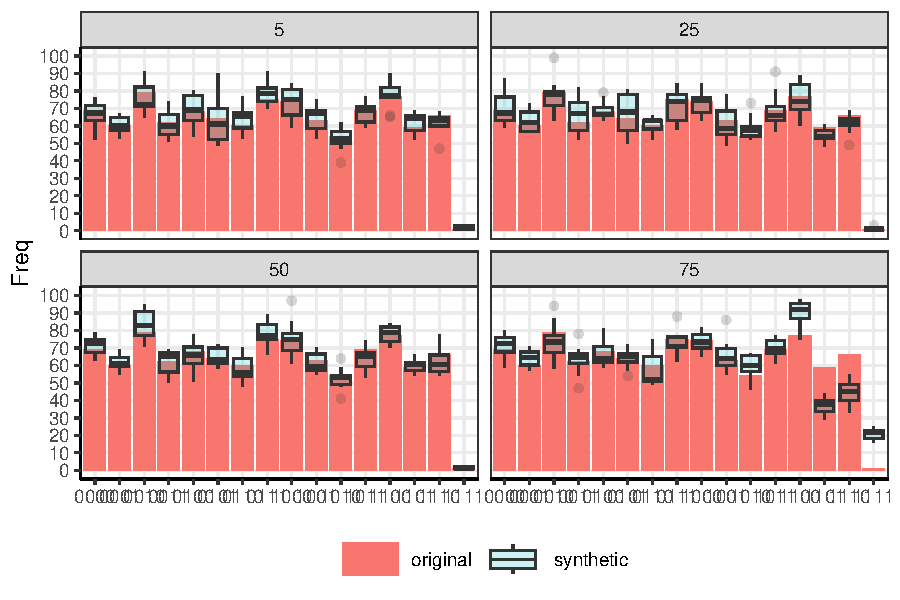
\includegraphics[width=\textwidth]{../../graphs/graph_cart_modified_mb_histogram_compare_10_v2.pdf}
        \caption{Minimum bucket (default is 5)}
        \label{fig:attacker_modified_mb_sensitivity}
    \end{subfigure}
    \hfill
    \begin{subfigure}{0.9\textwidth}
        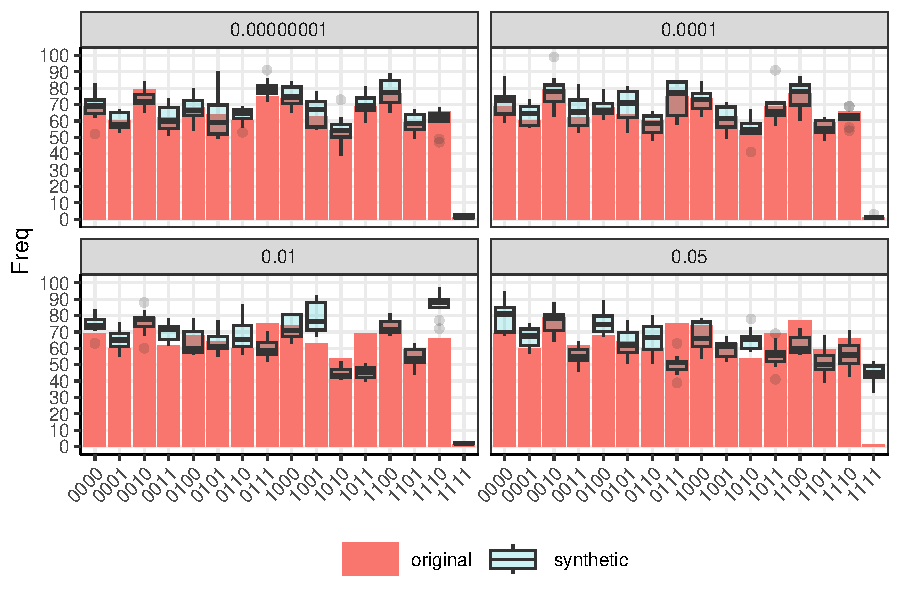
\includegraphics[width=\textwidth]{../../graphs/graph_cart_modified_cp_histogram_compare_10_v2.pdf}
        \caption{Complexity parameter (default is 10$^{-8}$)}
        \label{fig:attacker_modified_cp_sensitivity}
    \end{subfigure}
    \label{fig:compare_modified_sensitivity}
\end{figure}


\begin{table}[!h]
    \centering
    \caption{Risk measures for \texttt{depress} from keys: \texttt{sex}, \texttt{age}, \texttt{region}, \texttt{placesize} (SD2011)}
    % \rowcolors{1}{white}{lightgray}
    % latex table generated in R 4.4.0 by xtable 1.8-4 package
% Thu Feb 27 14:39:11 2025
\begin{tabular}{lrrrr}
   
\toprule & 
\multicolumn{2}{l}{Identity risk} &
\multicolumn{2}{l}{Attribute risk}
\\  
 
\cmidrule(lr){2-3}
\cmidrule(lr){4-5}
 
Data & Raab et al., 2024 & Modified & Raab et al., 2024 & Modified
\\ 

\midrule
Original data & 48.38 & 48.38 & 53.30 & 53.30 \\ 
  Synthetic 1 & 14.82 & 14.82 & 8.96 & 14.74 \\ 
  Synthetic 2 & 14.20 & 14.20 & 9.90 & 14.82 \\ 
  Synthetic 3 & 15.16 & 15.16 & 10.46 & 14.94 \\ 
  Synthetic 4 & 14.12 & 14.12 & 9.68 & 14.50 \\ 
  Synthetic 5 & 14.30 & 14.30 & 8.88 & 14.66 \\ 
  Average & 14.52 & 14.52 & 9.58 & 14.73 \\ 
   \bottomrule \\[-1.8ex] \multicolumn{5}{p{4in}}{Note: Modified indicates that values of \texttt{depress}=0  in synthetic data} 
\end{tabular}

    \label{tab:attribute_risk_sd2011}
\end{table}


\end{document}
